\documentclass[12pt,a4paper]{report}

% --- Paquetes de Idioma y Codificación ---
\usepackage[utf8]{inputenc}
\usepackage[T1]{fontenc}
\usepackage[spanish, es-tabla]{babel}

% --- Diseño de Página ---
\usepackage{geometry}
\geometry{top=2.5cm, bottom=2.5cm, left=3cm, right=3cm}

% --- Matemáticas y Símbolos ---
\usepackage{amsmath, amssymb, amsthm}

% --- Colores y Cajas ---
\usepackage[dvipsnames]{xcolor}
\usepackage[most]{tcolorbox}

% Caption

\usepackage{caption}

% Gráficos

\usepackage{graphicx}

% Espaciadora

\newcommand{\esp}{\vspace{0.5cm}}

% promedio

\newcommand{\prom}[1]{\left\langle #1 \right\rangle}

% ket

\newcommand{\ket}[1]{| #1 \rangle}

% bra

\newcommand{\bra}[1]{\langle #1 |}

% braket

\newcommand{\braket}[2]{\langle #1 | #2 \rangle}

% Bibliografía

\usepackage[style=apa, backend=biber]{biblatex} % Estilo APA
\addbibresource{biblio.bib} % Nombre de tu archivo .bib

% Configuración de cajas personalizadas
\newtcolorbox{importante}{
	colback=red!5!white,
	colframe=red!75!black,
	title=Importante,
	fonttitle=\bfseries
}

\newtcolorbox{nota}{
	colback=blue!5!white,
	colframe=blue!75!black,
	title=Nota,
	fonttitle=\bfseries
}

% Definición de la caja de bibliografía
\newtcolorbox{bibliografia}{
	colback=gray!5!white,
	colframe=gray!75!black,
	title=Bibliografías útiles,
	fonttitle=\bfseries,
	breakable
}

% Socrative para óptica 2

\newtcolorbox{Socrative}{
	colback=orange!5!white,
	colframe=orange!75!black,
	title=Socrative,
	fonttitle=\bfseries,
	breakable
}

% Float

\usepackage{float}

% --- Hipervínculos ---
\usepackage{hyperref}
\hypersetup{
	colorlinks=true,
	linkcolor=blue,
	filecolor=magenta,      
	urlcolor=cyan,
}

% --- Datos del Documento ---
\title{Óptica II}
\author{Chengyu Jin}
\date{\today}

\begin{document}
	
	\maketitle
	
	\tableofcontents
	\newpage
	
	\chapter{Teoría escalar de la Difracción. Difracción de campo lejano y de campo cercano. Redes de difracción.}
	
	\begin{bibliografia}
		\begin{enumerate}
			\item Casas, J. ''Óptica''. Cap. 10,11
			\item Pedrotti, F.L., Pedrotti, L.S. ''Introduction to Optics''. Cap. 16-18
			\item Nieves, J.L, Jiménez, J.R. y Hernández-Andrés, J. ''Introducción a la teoría difraccional de la formación de imágenes''. Cap. 2,3
			\item Hecht-Zajac- ''Óptica''. Cap.10.
			\item Klen, M.V., Furtak, T.E. ''Optics''. Cap.6
			\item Malacara, D. ''Óptica básica''. Cap. 10-11
			\item Jenkins, F.A., White, H.E. ''Fundamentals of Optics''. Cap. 15-18
			\item Goodman. J. ''Introduction to Fourier Optics'', Cap. 4
			\item Born, M., Wolf, E. ''Principles of Optics.'' Cap. 8
		\end{enumerate}
	\end{bibliografia}
	
	\section{Teoría escalar de la difracción}
	
	La difracción fue uno de los últimos grandes fenómenos ópticos en observarse: el primer experimento conocido data de 1648, cuando Francesco de Grimaldi publica un tratado tras observar que en determinadas condiciones experimentales existía luz dentro de la zona de sombra geométrica proyectada por un obstáculo en una pantalla opaca.
	
	\esp
	
	La luz entonces se ha desviado de su trayectoria rectilínea prevista por la óptica geométrica para \textit{invadir} la zona de sombra. Grimaldi estableció que el fenómeno observado se debía a un modo de propagación de la luz que denominó \textit{diffractio} (del latín \textit{diffractus} que significa rotura o quiebra), diferente de la reflexión y la refracción, ya conocidas por el modelo geométrico. Esta definición es sorprendentemente similar a la más moderna proporcionada por Sommerfield (uno de los científicos que ha contribuido de forma importante a modelizar la difracción), que dice que la difracción es
	
	\begin{quote}
		\textit{Toda desviación de la trayectoria rectilínea de la luz no debida a reflexión o refracción.}
	\end{quote}
	
	No siempre que la luz encuentre un obstáculo en su camino vamos a poder observar patrones de difracción (si no, sería bastante difícil desenvolverse en el mundo que nos rodea, al igual que si observásemos interferencias siempre que se superpusieran dos fuentes en algún punto del espacio). La difracción vamos a poder observarla en especial cuando la fuente sea bastante coherente, y el obstáculo que cercena el frente de ondas muy pequeño (tomando como referencia la longitud de onda media de la fuente, puede ser de algunos órdenes de magnitud superior, pero no mucho más).
	
	\esp
	
	Vemos algunos ejemplos más de patrones obtenidos con fuentes coherentes y orificios pequeños. Esto puede servir para complementar la observación directa de patrones producidos con un puntero láser y un pelo, o un CD. Se produce una redistribución espacial de la energía emitida por la fuente para conformar estos patrones, de forma similar (aunque se trata de un fenómeno bien distinto como veremos) a cuando se produce un patrón de interferencias. En muchas ocasiones, interferencias y difracción se producen conjuntamente, y veremos cómo la teoría descriptiva de los patrones difractivos que explicamos en el tema será capaz también de describir los patrones interferenciales en estos casos.
	
	\subsection{Teoría de Kirchhoff}
	
	\begin{figure}[H]
		\centering
		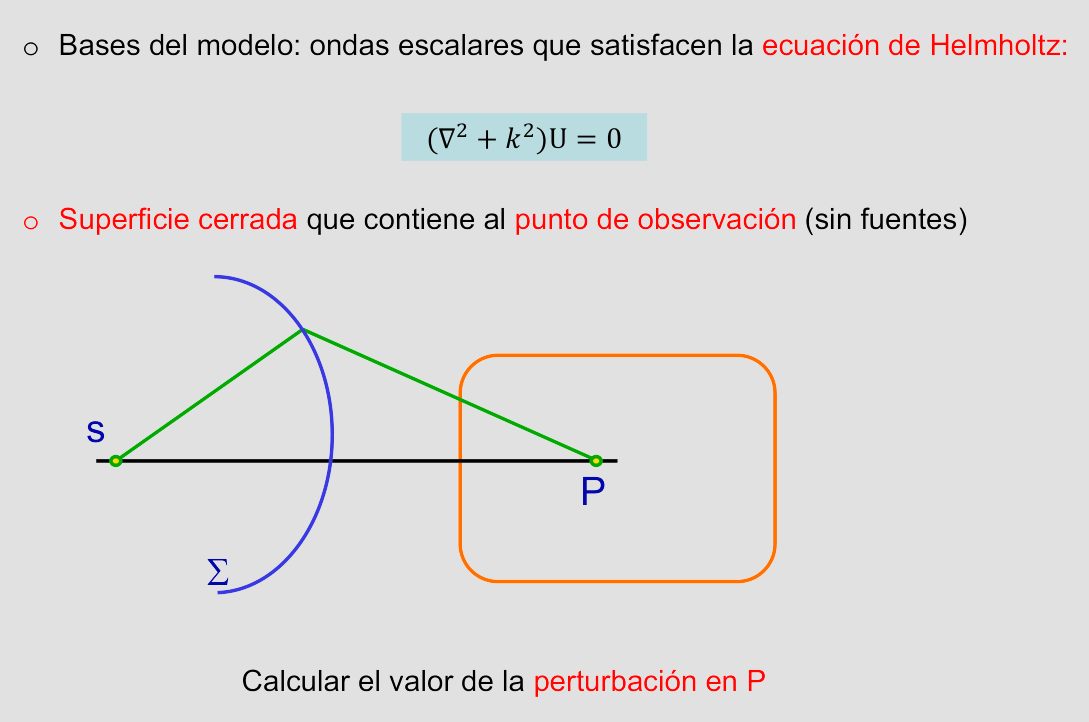
\includegraphics[width=0.7\textwidth]{IMG/teoriakirch.png}
	\end{figure}
	
	\esp
	
	Kirchhoff dedujo sus resultados fundamentales a partir de la ecuación de ondas escalar. Por eso se enmarca este modelo en el grupo de resultados denominado \textit{teoría escalar de la difracción}. Funciona bien la \textbf{aproximación escalar} para la difracción si las dimensiones de la \textbf{abertura son grandes} comparadas con la \textbf{longitud de onda de la onda difractada}, pues entonces la interacción de los campos $\vec{E}$ y $\vec{H}$ se extiende sólo al rango de unas cuantas longitudes de onda en torno a los bordes de la abertura, y no habrá efectos de acoplamiento de condiciones de contorno para ambos campos.
	
	\esp
	
	Esto es equivalente a suponer que desde la fuente y desde el punto de observación, los ángulos hasta los bordes de la abertura son pequeños. Debemos tener presente entonces que estamos realizando una aproximación, y su rango de validez. Pero la simplificación que supone hace que esta teoría resulte muy ventajosa en la mayoría de casos y situaciones experimentales.
	
	\esp
	
	En esta seccion, explicamos sus principios y resultados básicos. También comentaremos brevemente en las actividades de clase la evolución posterior debida a Sommerfeld y Rayleigh, y cómo ésta soluciona a su vez los problemas que presenta el modelo de Kirchhoff.
	
	\esp
	
	El planteamiento de Kirchhoff es bastante original. Parte de la ecuación de ondas escalar o ecuación de Helmholtz, que se deduce a partir de la ecuación de ondas para un campo escalar. Para un campo escalar que verifique la \textbf{ecuación de Helmholtz}, Kirchoff propone considerar una superficie cerrada que contiene al punto de observación $P$ (pero sin fuentes dentro) y para la cual se supone conocido en todos sus puntos el valor de la función de onda procedente de la fuente y su derivada en dirección normal a la superficie. El problema consiste entonces en encontrar el valor de la función procedente de la fuente en $P$ (tras pasar por la abertura difractante) a partir de estos valores conocidos.
	
	\esp
	
	\begin{equation}
		(\nabla^2+k^2)U=0
	\end{equation}
	
	\esp
	
	\begin{figure}[H]
		\centering
		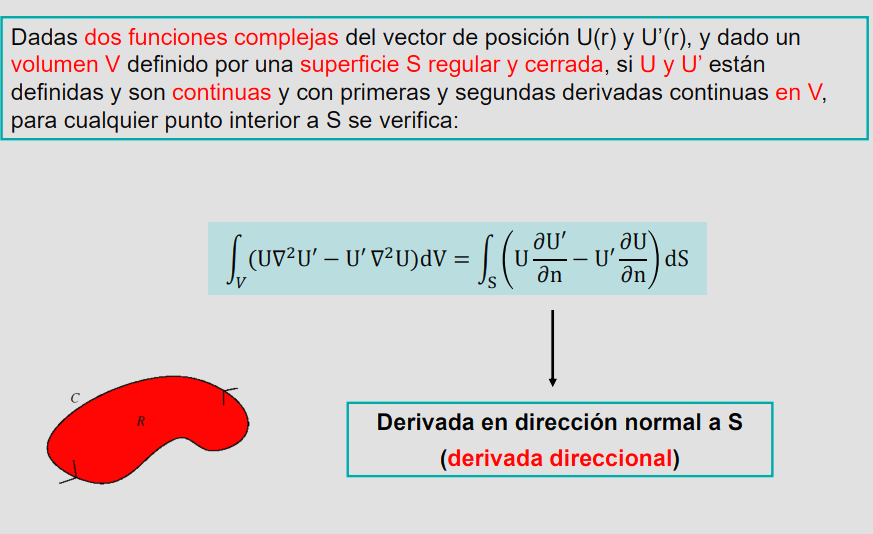
\includegraphics[width=0.7\textwidth]{IMG/verde.png}
	\end{figure}

	\esp
	
	\noindent Las dos bases fundamentales de la teoría de Kirchhoff son entonces la ecuación de ondas escalar de Helmholtz, que ya hemos mostrado, y el Teorema de Green, cuyo enunciado dice:
	
	\esp
	
	\begin{quote}
		dadas dos funciones complejas del vector posición, $U(r)$ y $U'(r)$, y dado un volumen $V$ definido por una superficie $S$ regular y cerrada, si $U(r)$ y $U'(r)$ están definidas y son continuas y con primeras derivadas continuas en $V$, entonces para cualquier punto interior a $S$ se verifica la siguiente relación:
	\end{quote}
	
	\esp
	
	\begin{equation*}
		\int_V (u\nabla^2u' - u'\nabla^2u) \, dV = \int_S \left( u\frac{\partial u'}{\partial n} - u'\frac{\partial u}{\partial n} \right) \, dS %
	\end{equation*}
	
	\esp
	
	Recordamos el significado de una superficie regular y cerrada. Por ejemplo, una esfera es regular pero un cubo no lo es, porque presenta discontinuidades en los vértices. 
	
	\esp
	
	\begin{figure}[H]
		\centering
		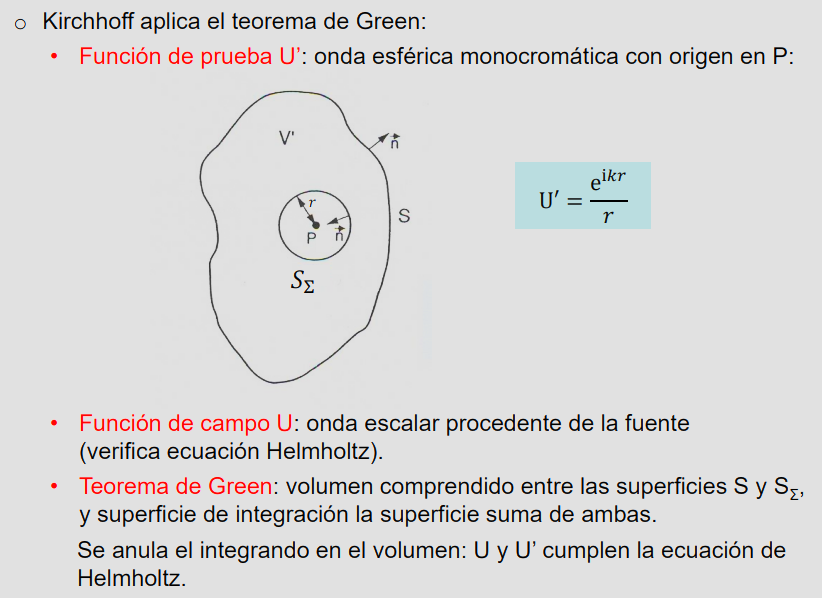
\includegraphics[width=0.7\textwidth]{IMG/teoriakirch2.png}
	\end{figure}
	
	\esp
	
	Vamos a ir concretando ya la aplicación que Kirchhoff hizo de este teorema. En primer lugar, tomamos una superficie cerrada que rodea a $P$ (por el momento, nos vamos a olvidar de que la luz de la fuente llega a una abertura difractante). Como función de prueba $U'$ para aplicar el teorema de Green, Kirchhoff toma una función que sería similar en forma a una onda monocromática esférica con origen de $P$, pero en realidad no debemos perder de vista que la función de prueba es una herramienta puramente matemática y no tiene por qué tener significado físico, como veremos hacia el final del tema en especial.
	
	\esp
	
	\begin{equation}
		U' =\frac{e^{ikr}}{r}
	\end{equation}
	
	\esp
	
	Ya sabemos que $U'$ y su derivada normal en $S$ deben estar definidas y ser continuas en todo $V$, así que se nos plantea el problema de la discontinuidad de $U'$ en $P$. Para soslayarlo, lo que hacemos es tomar una segunda superficie esférica $\Sigma$ de radio $r'$ tan reducido como queramos, que rodea a $P$. Aplicaremos el teorema de Green al volumen $V$ comprendido entre las superficies $S$ y $\Sigma$, y la superficie de integración será la superficie suma de ambas (superficie de dos hojas). Como función $U$, tomamos la onda procedente de la fuente, cuyo valor en $P$ pretendemos conocer.

	\printbibliography[title={Bibliografía}]
\end{document}